% \partapendices
%%% https://www.codecogs.com/latex/eqneditor.php?lang=pt-br
% \begin{equation}
%     \alpha = \sum_{i=0}^{\infty}{a_i x^i}
% \end{equation}

% \begin{equation}
%     \beta = \sum_{i=0}^{\infty}{a_i x^{2\pi i}\frac{\partial^2 }{\partial x^2}}f(xi)
% \end{equation}

\begin{apendicesenv}
\partapendices
\chapter{Requisitos}
\label{apice:requisitos_unificados}

Este apêndice apresenta a consolidação integral dos requisitos técnicos levantados e unificados pelas frentes de Estrutura, Eletrônica, Software e Energia do projeto Micromouse. O agrupamento elimina redundâncias e estabelece a rastreabilidade direta entre as restrições físicas do robô e as metas de navegação autônoma.

\vspace{1em}

\small
\begin{longtable}{|p{0.08\textwidth}|p{0.25\textwidth}|p{0.45\textwidth}|p{0.14\textwidth}|}
    \caption{Listagem integral dos Requisitos Funcionais (RF) e Não-Funcionais (RNF) unificados.}
    \label{tab:requisitos_unificados_integral} \\
    
    \hline
    \textbf{ID} & \textbf{Nome do Requisito} & \textbf{Descrição Técnica} & \textbf{Origem} \\ \hline
    \endfirsthead
    
    \multicolumn{4}{c}%
    {\tablename\ \thetable\ --- \textit{Continuação da página anterior}} \\
    \hline
    \textbf{ID} & \textbf{Nome do Requisito} & \textbf{Descrição Técnica} & \textbf{Origem} \\ \hline
    \endhead
    
    \hline \multicolumn{4}{r}{\textit{Continua na próxima página...}} \\
    \endfoot
    
    \hline
    \endlastfoot
    
    \multicolumn{4}{|l|}{\textbf{1. Requisitos Funcionais (RF)}} \\ \hline
    
    \textbf{RF01} & Detecção de Paredes e Obstáculos & O sistema deve detectar paredes do labirinto e obstáculos nas direções frontal, esquerda e direita durante a navegação, distinguindo corretamente paredes brancas do piso preto. & Eletrônica + Software \\ \hline
    
    \textbf{RF02} & Localização e Navegação Autônoma & O robô deve calcular sua posição, orientação e deslocamento dentro de um labirinto de até 16×16 células utilizando sensores e odometria. & Eletrônica + Software + Estrutura \\ \hline
    
    \textbf{RF03} & Execução Local da Navegação & Toda a lógica de navegação, exploração e resolução do labirinto deve ser executada localmente no robô, sem dependência de processamento externo. & Eletrônica \\ \hline
    
    \textbf{RF04} & Armazenamento do Mapa & O sistema deve possuir memória suficiente para armazenar e atualizar a representação de um labirinto de até 16×16 células. & Eletrônica \\ \hline
    
    \textbf{RF05} & Comunicação e Telemetria & O sistema deve manter comunicação sem fio com um servidor para transmissão de telemetria em tempo real durante o percurso. & Eletrônica + Software \\ \hline

    \multicolumn{4}{|l|}{\textbf{2. Requisitos Não-Funcionais (RNF)}} \\ \hline
    
    \textbf{RNF01} & Latência de Transmissão & O sistema deve processar e despachar os pacotes de telemetria com latência ponta a ponta que assegure a responsividade da interface. & Eletrônica + Software \\ \hline

    \textbf{RNF02} & Confiabilidade Sem Fio & A comunicação sem fio deve manter perda de pacotes inferior a 5\% durante a operação em labirintos de até 16×16 células. & Eletrônica \\ \hline

    \textbf{RNF03} & Estabilidade de Sinais & O sistema eletrônico deve garantir a integridade da leitura dos sensores analógicos e digitais sob condições dinâmicas de operação. & Eletrônica \\ \hline

    \textbf{RNF04} & Autonomia Energética & O sistema deve possuir autonomia mínima suficiente para executar pelo menos 3 execuções completas do labirinto sem recarga. & Eletrônica + Energia \\ \hline
    
    \textbf{RNF05} & Limite Dimensional & A largura operacional do robô deve ser menor ou igual a 10 cm para permitir manobras seguras. & Estrutura \\ \hline
    
    \textbf{RNF06} & Massa Total & A massa total do robô deve ser menor ou igual a 250 g. & Estrutura \\ \hline
    
    \textbf{RNF07} & Estabilidade Mecânica & O centro de massa deve permanecer abaixo de 2 cm de altura e até 1,5 cm à frente do eixo motriz. & Estrutura \\ \hline
    
    \textbf{RNF08} & Aderência da Tração & O sistema de tração deve garantir coeficiente de atrito mínimo equivalente a $\mu \geq 0,7$. & Estrutura \\ \hline
    
    \textbf{RNF09} & Rigidez Estrutural & Os suportes dos sensores devem apresentar deformação inferior a 0,1 mm sob carga de 2 N. & Estrutura \\ \hline

\end{longtable}

% --- APÊNDICE C ---
\chapter{Roteiro de Testes Funcionais}
\label{apice:roteiro_testes}

Apresenta-se a seguir a listagem detalhada dos casos de teste (TF) projetados para validar as funcionalidades do ecossistema de \textit{software} do Micromouse, garantindo o atendimento aos requisitos funcionais e não-funcionais.

\vspace{1em}

\small
\begin{longtable}{|p{0.08\textwidth}|p{0.18\textwidth}|p{0.22\textwidth}|p{0.22\textwidth}|p{0.18\textwidth}|}
    \caption{Roteiro de validação funcional do sistema de telemetria e dashboard.}
    \label{tab:roteiro_testes_integral} \\
    
    \hline
    \textbf{Cód.} & \textbf{Nome/Objetivo} & \textbf{Pré-condições} & \textbf{Procedimentos} & \textbf{Resultado Esperado} \\ \hline
    \endfirsthead
    
    \multicolumn{5}{c}%
    {\tablename\ \thetable\ --- \textit{Continuação da página anterior}} \\
    \hline
    \textbf{Cód.} & \textbf{Nome/Objetivo} & \textbf{Pré-condições} & \textbf{Procedimentos} & \textbf{Resultado Esperado} \\ \hline
    \endhead
    
    \hline \multicolumn{5}{r}{\textit{Continua na próxima página...}} \\
    \endfoot
    
    \hline
    \endlastfoot
    
    \textbf{TF01} & Validar visualização em tempo real & ESP32 conectado e transmitindo dados. & Abrir Dashboard e observar a atualização do ícone do robô. & O mapa deve atualizar com latência inferior a 150 ms. \\ \hline
    
    \textbf{TF02} & Validar detecção de paredes & Robô posicionado no labirinto de teste. & Executar movimento e observar a grade no Dashboard. & Paredes devem aparecer na interface conforme leitura dos ToFs. \\ \hline
    
    \textbf{TF03} & Validar estados da FSM & Firmware operando normalmente. & Disparar transições (ex: MAPPING para ERROR). & O \textit{badge} de estado deve refletir a Tag \texttt{estado\_robo}. \\ \hline
    
    \textbf{TF04} & Validar telemetria odométrica & Sensores e encoders calibrados. & Movimentar o robô por 18 cm. & Os campos \texttt{pos\_x} e \texttt{pos\_y} devem atualizar corretamente. \\ \hline
    
    \textbf{TF05} & Validar estabilidade WebSocket & Servidor Backend em execução. & Manter conexão ativa por 10 minutos de prova. & O sistema deve manter o fluxo sem quedas ou perda de pacotes > 5\%. \\ \hline
    
    \textbf{TF06} & Validar persistência InfluxDB & Sessão de corrida concluída. & Consultar o banco via interface administrativa. & Measurement \texttt{log\_corrida} deve conter os dados vinculados ao \texttt{id\_corrida}. \\ \hline
    
    \textbf{TF07} & Validar consulta histórica & Banco de dados com múltiplas corridas. & Utilizar o seletor de histórico no Dashboard. & A interface deve carregar trajetos de execuções passadas com sucesso. \\ \hline
    
    \textbf{TF08} & Validar exportação de dados & Logs disponíveis no servidor. & Clicar no botão "Exportar" na interface. & Download de arquivo CSV ou JSON estruturado e válido. \\ \hline
    
    \textbf{TF09} & Validar troca de modos & Robô transitando para \texttt{FAST\_RUN}. & Observar a alteração dinâmica dos widgets. & A interface deve priorizar velocidade e tempo em detrimento do mapa exploratório. \\ \hline
    
    \textbf{TF10} & Validar buffer local & Perda súbita de Wi-Fi durante a prova. & Desconectar o ponto de acesso Wi-Fi. & O robô deve armazenar métricas criticamente em memória local temporária. \\ \hline
    
    \textbf{TF11} & Validar sincronização pós-falha & Buffer local preenchido e rede restaurada. & Reestabelecer o sinal Wi-Fi. & O sistema deve despachar os dados pendentes ordenados pelo campo \texttt{time}. \\ \hline
    
    \textbf{TF12} & Validar monitoração energética & ADC da bateria conectado ao ESP32. & Consumir carga e observar o Dashboard. & O campo \texttt{bateria} deve exibir valores em Volts com precisão de uma casa decimal. \\ \hline
    
    \textbf{TF13} & Validar áreas inexploradas & Início da fase \texttt{MAPPING}. & Observar o contraste visual da grade. & Células não visitadas devem possuir preenchimento visual distinto. \\ \hline
    
    \textbf{TF14} & Validar carga assíncrona & Fluxo intenso de telemetria em 16x16. & Enviar 50 pacotes/segundo para o Dashboard. & A interface web deve permanecer responsiva aos comandos do desenvolvedor. \\ \hline

\end{longtable}

\chapter{Maquina de Estados}
\label{apice:maquina_de_estados}
\begin{figure}[htbp]
        \centering
        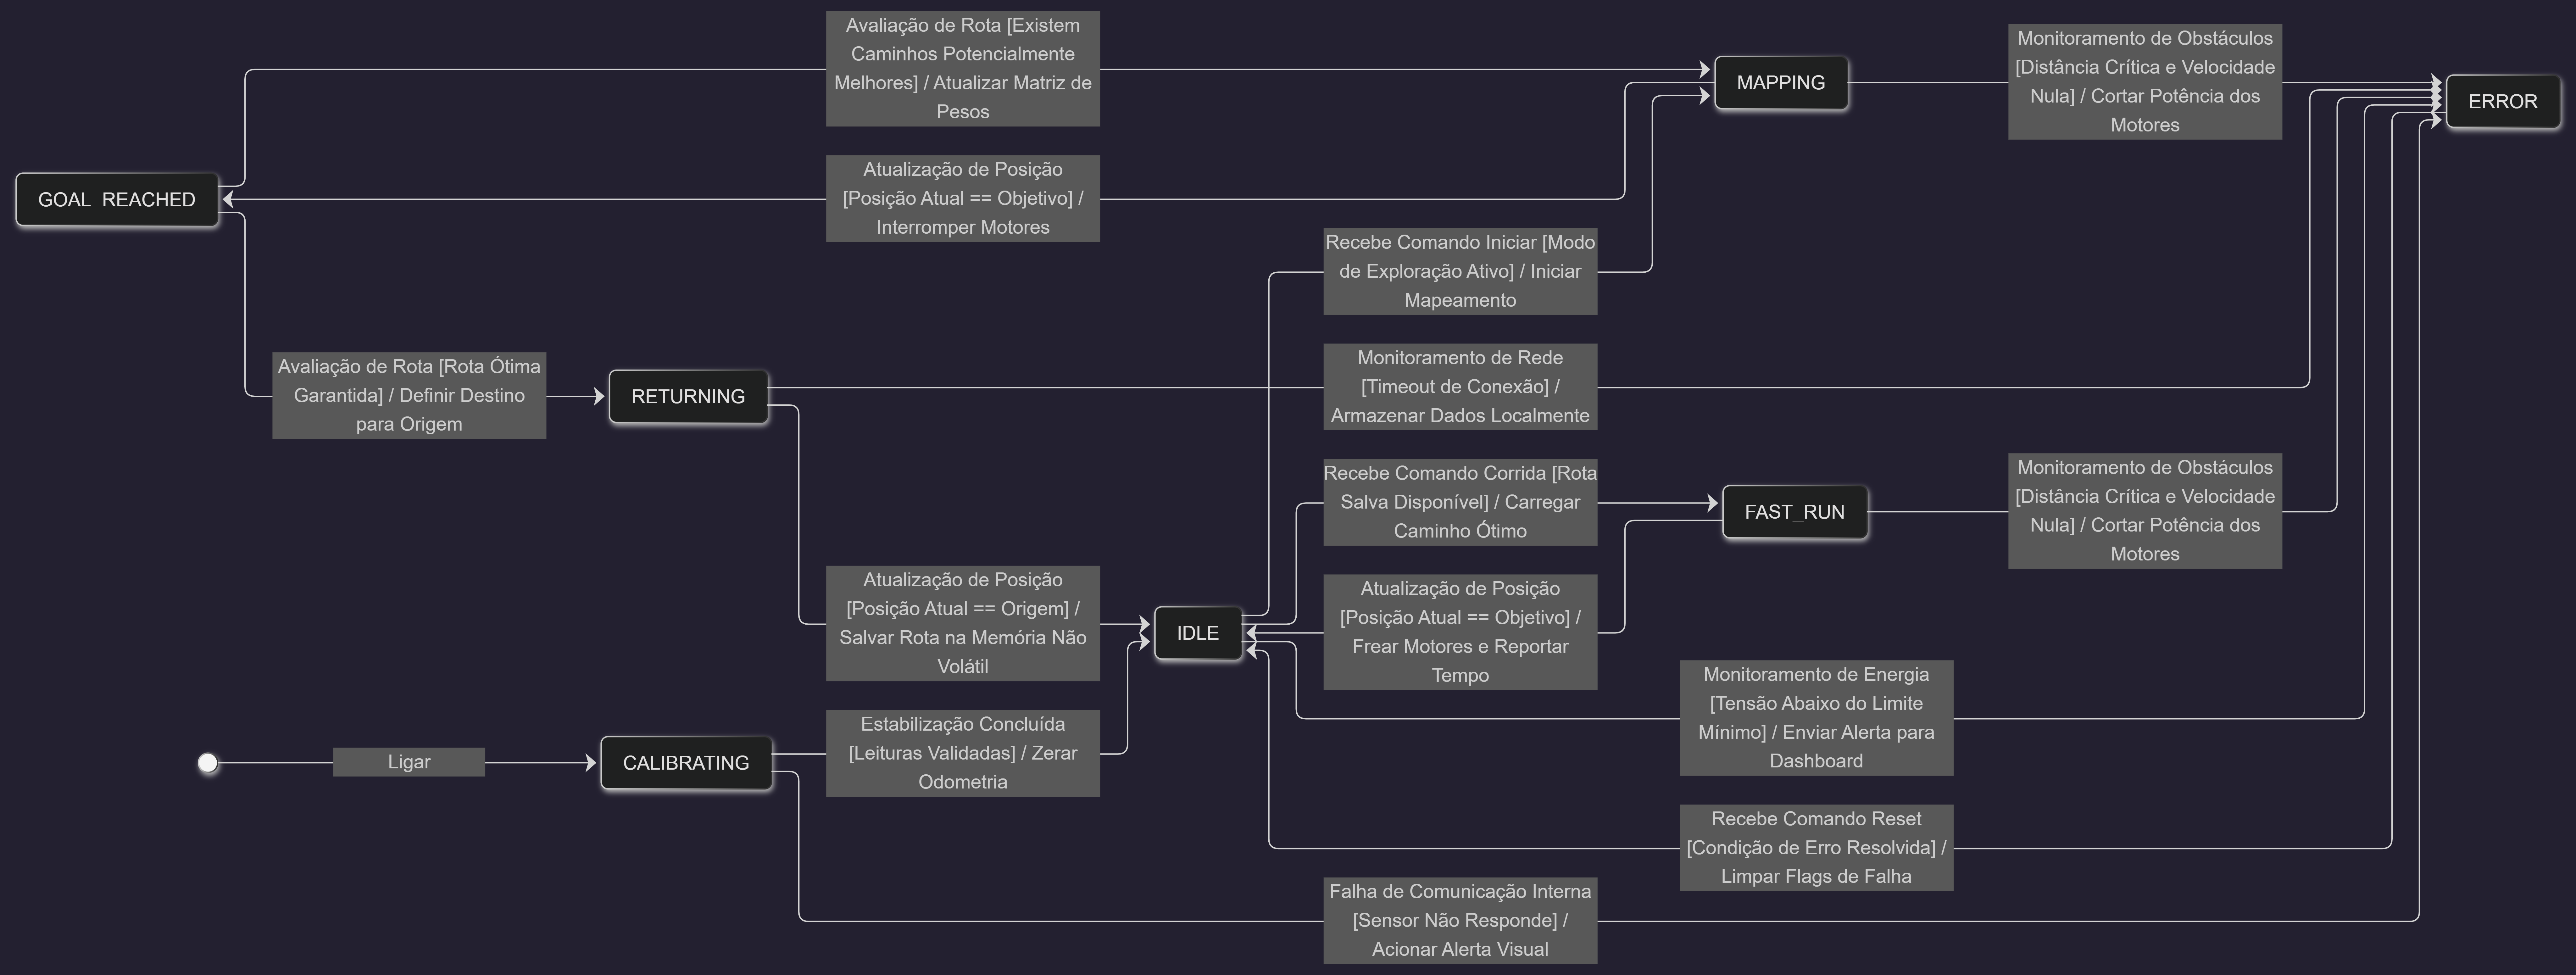
\includegraphics[width=0.8\textwidth]{figuras/maquina_de_estados.png}
        \caption{Diagrama de Estados do Firmware (FSM).}
        \label{fig:diagrama_estados}
    \end{figure}

\chapter{Desenhos técnicos Estruturais}
\label{APÊNDICE E}
\begin{figure}[htbp]
        \centering
        \includegraphics[width=1\textwidth]{figuras/Code_Generated_Image.eps}
        \caption{Desenho esquemático do labirinto de testes com o posicionamento dos postes}
        \label{fig:Desenho esquematoco do Labirinto de Testes}
    \end{figure}

\begin{figure}[htbp]
        \centering
        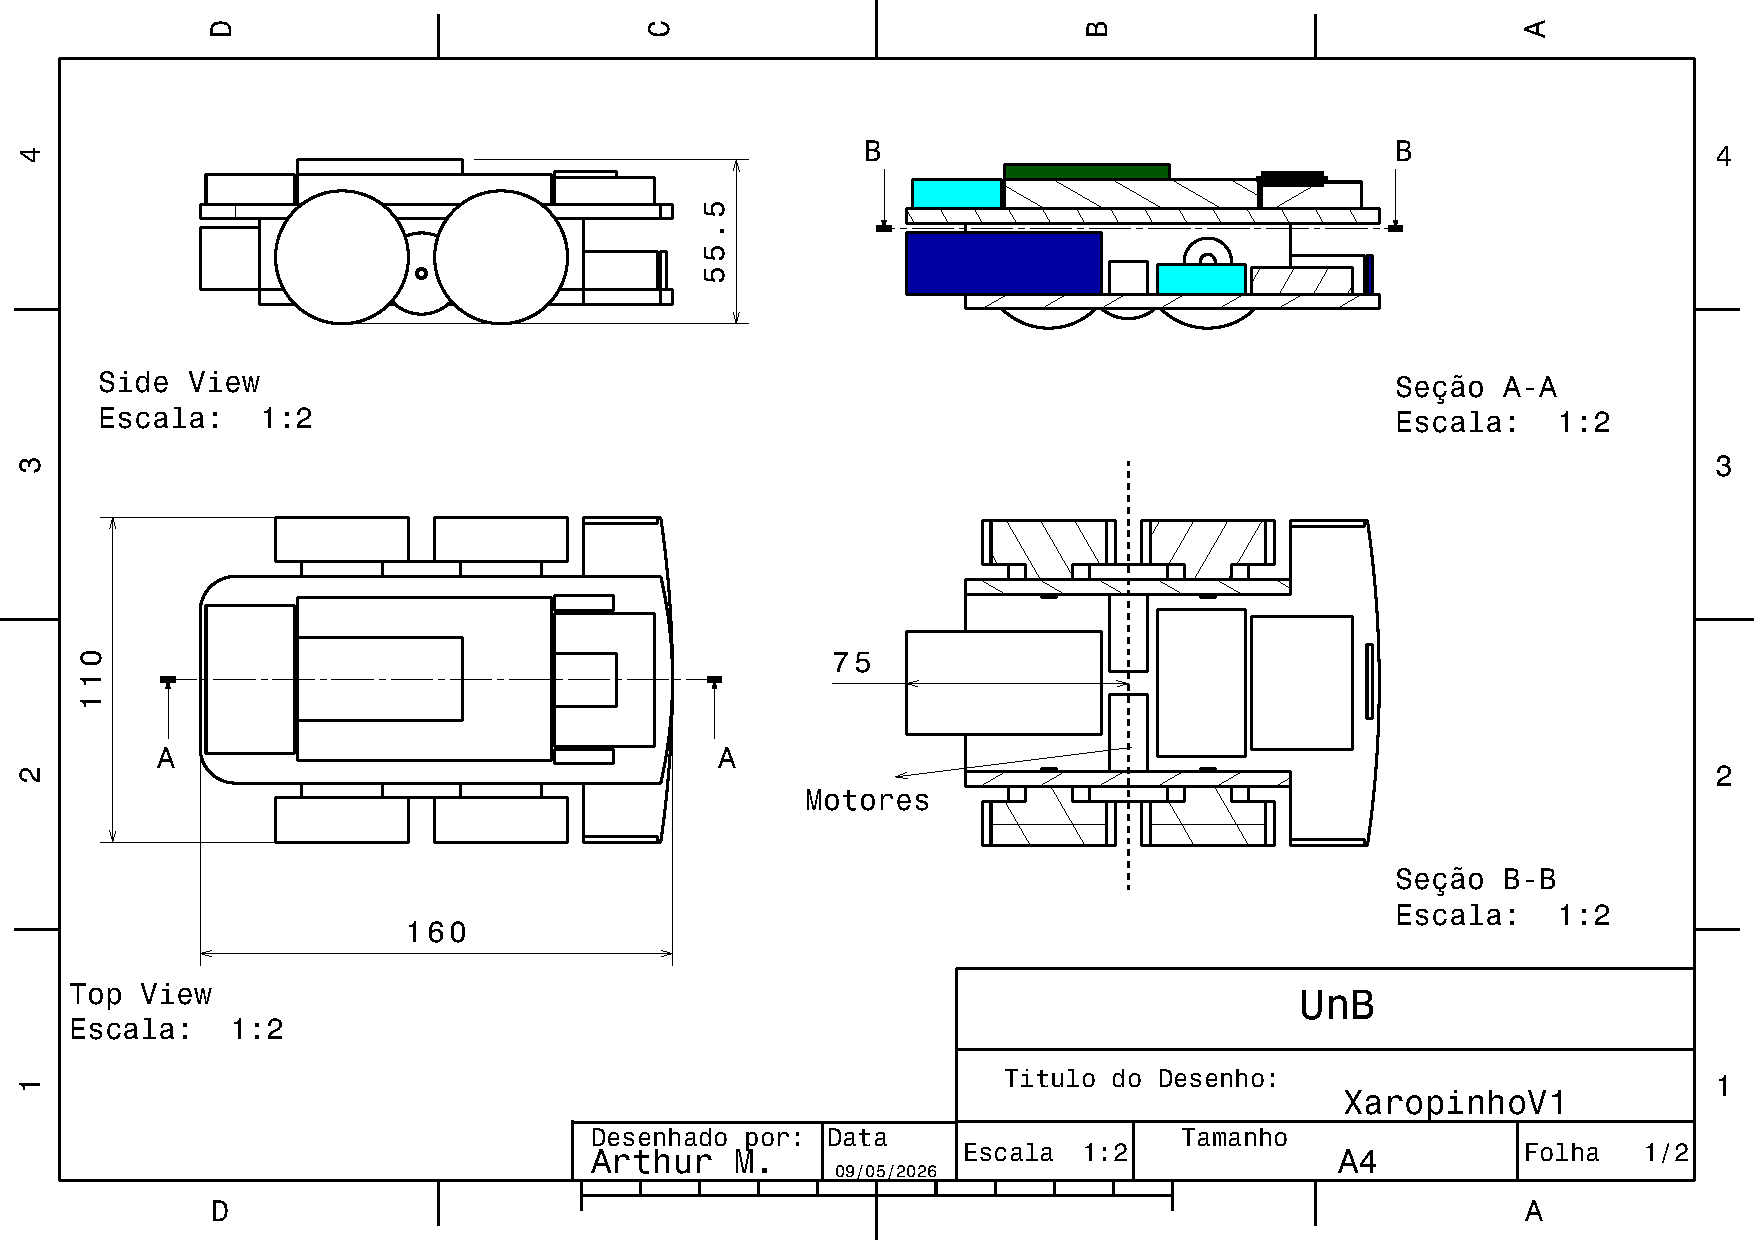
\includegraphics[width=1\textwidth]{editaveis/DraftXaropinhoV1_Sheet_1.pdf}
        \caption{Detalhamento dimensional e estrutural do robô em escala 1:2}
        \label{fig:Draft Micromouse}
    \end{figure}

    \begin{figure}[htbp]
        \centering
        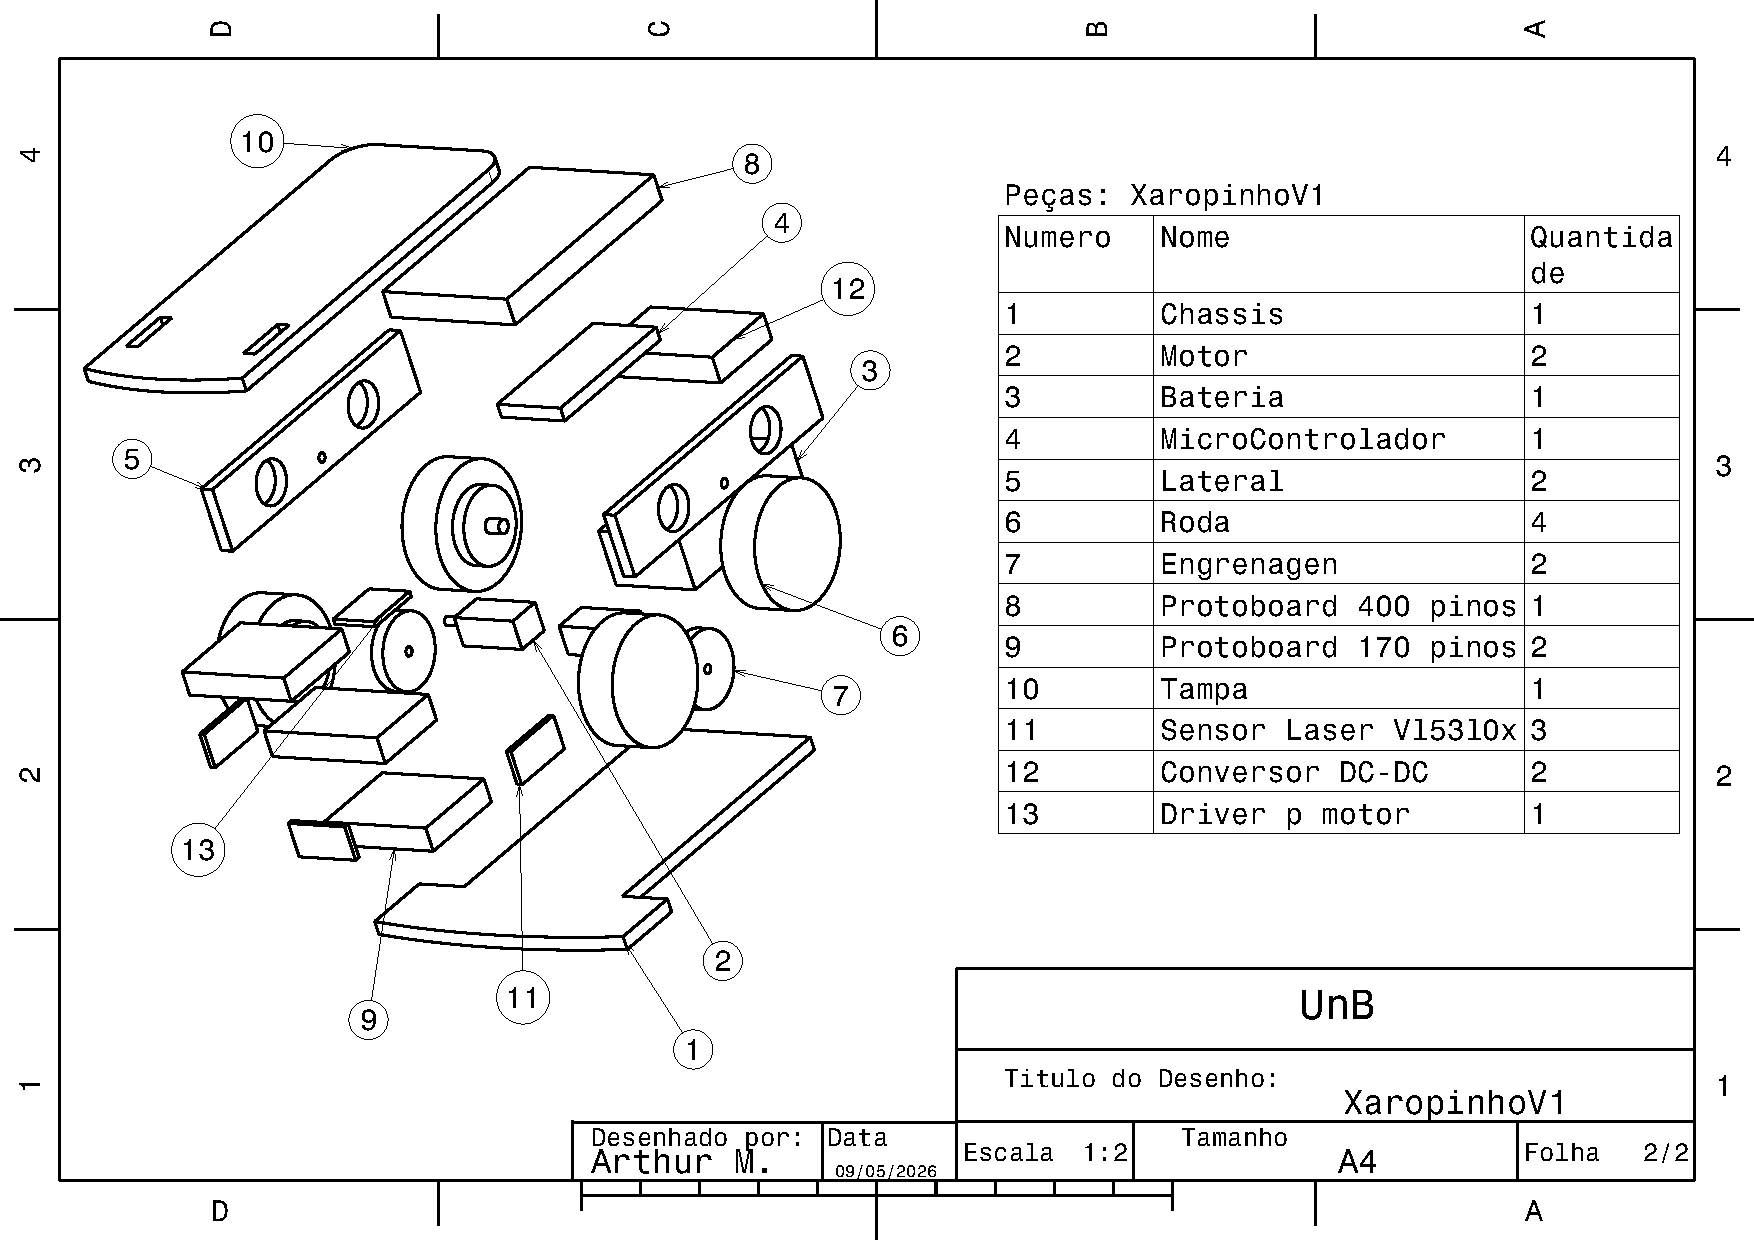
\includegraphics[width=1\textwidth]{editaveis/DraftXaropinhoV1_Sheet_2.pdf}
        \caption{Vista explodida do Micromouse com hierarquia de montagem e a integração entre os subsistemas mecânicos e eletrônicos}
        \label{fig:Draft Micromouse explodido}
    \end{figure}

    \begin{figure}[htbp]
        \centering
        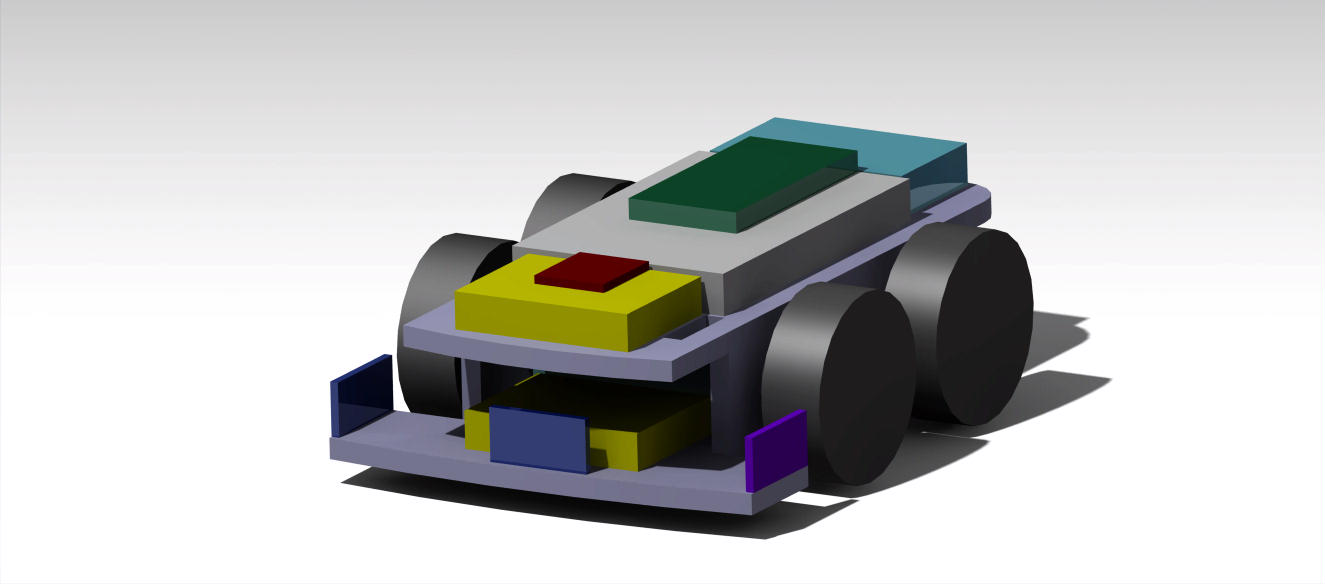
\includegraphics[width=1\textwidth]{editaveis/IsoRender.jpg}
        \caption{Renderização isométrica do modelo CAD detalhando a disposição modular dos componentes e a estrutura do chassi.}
        \label{fig:iso do micromouse}
    \end{figure}
    
\end{apendicesenv}



